\documentclass{article}[11pt]
\usepackage{graphicx}   % Including figure files
\usepackage{caption}
\setlength{\textwidth}{17cm}
\setlength{\hoffset}{-2cm}
\begin{document}
\begin{figure}
 \begin{minipage}[c]{0.6\textwidth}
  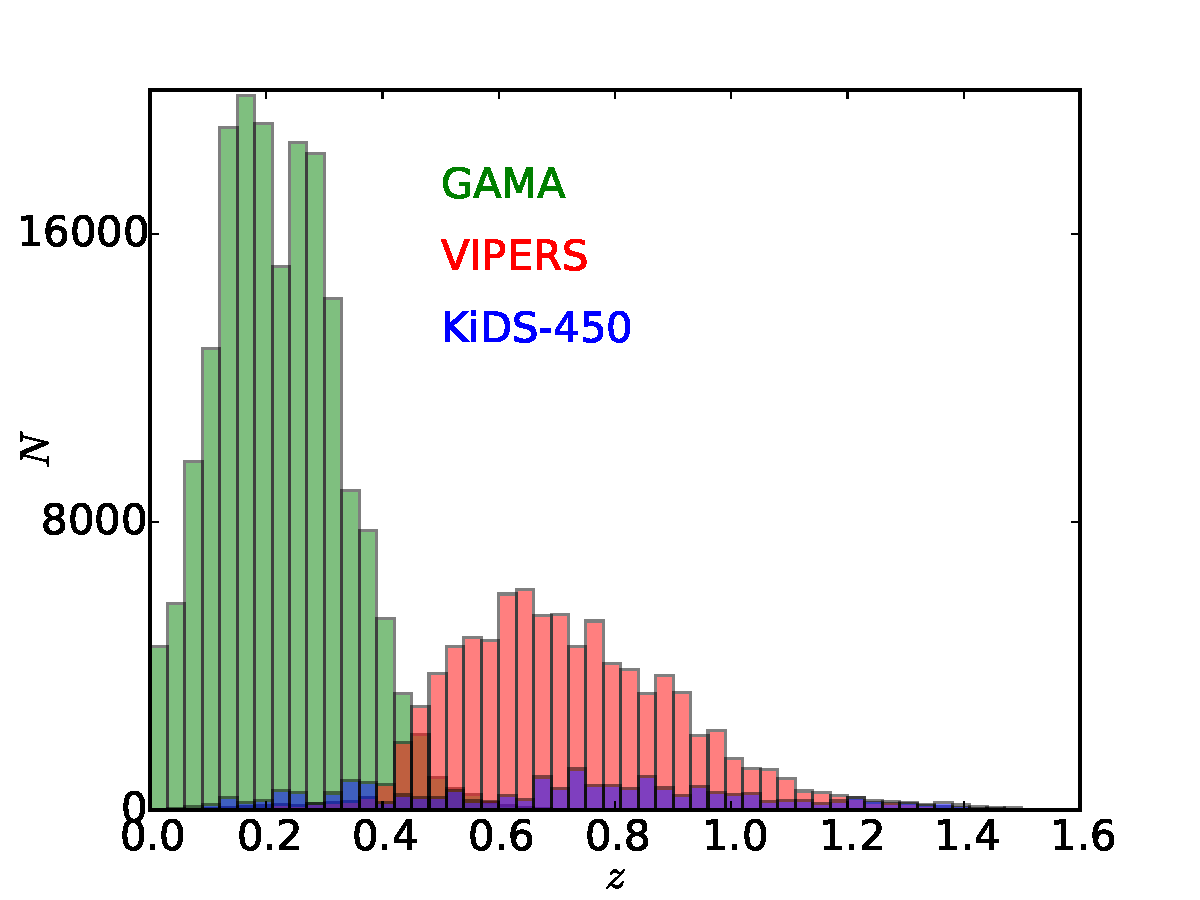
\includegraphics[width=\textwidth]{ESO_prop_plot_zdist.pdf}
  \end{minipage}\hfill
  \begin{minipage}[c]{0.35\textwidth}
    \caption*{Fig.~2: Numbers of spectroscopic redshifts available in GAMA, VIPERS and SDSS-BOSS, vs. the number that were used in the KiDS-450 CC calibration of Hildebrandt et al. (2017). GAMA and SDSS overlap with KiDS and will be used at $z<0.7$; with the proposed KiDS/VIKING-like imaging of the VIPERS area we will be able to do the same at higher redshift.}
  \end{minipage}
\end{figure}
\end{document}
